\documentclass[11pt]{article}
\usepackage[a4paper,margin=2.3cm]{geometry}
\usepackage[T1]{fontenc}
\usepackage{lmodern}
\usepackage{booktabs}
\usepackage{graphicx}
\usepackage{amsmath}
\usepackage{float}
\usepackage[font=small]{caption}
\usepackage{enumitem}
\usepackage{fancyvrb}
\usepackage[hidelinks]{hyperref}
\setlist{itemsep=1pt,topsep=3pt}
\fvset{fontsize=\scriptsize,frame=single,framesep=2mm}

\title{Software-Defined Networking\\[2pt]\large Assignment 3 --- COL7524}
\author{Entry numbers: 2026MCS2494, 2026MCS2493}
\date{}

\begin{document}
\maketitle

% =====================================================================
\section{Setup}

\subsection{Environment}
Everything runs on one Windows 11 laptop inside WSL2 (Ubuntu 24.04). Mininet 2.3.0, Open vSwitch
3.3.9 and iperf 2.1.9 come from apt. Ryu 4.34 does not run on Ubuntu's Python 3.12, so it lives in
its own Python 3.9 virtual environment (\texttt{\textasciitilde/ryu-env}) with eventlet pinned to
0.30.2 and setuptools to 67.6.1 --- newer versions of either break Ryu. All switches speak
OpenFlow 1.3 and the controller always listens on \texttt{127.0.0.1:6633}.

\subsection{Topologies and changes}
Part 1 uses \texttt{p1\_topo.py} unchanged. Parts 2 and 3 use \texttt{Part 2/p2\_topo.py}, which builds
exactly the ring of \texttt{p3\_topo.py} but reads the bandwidth and delay of every ring link from a
JSON file. The point of this is that the topology and the controller read the \emph{same} numbers,
so the controller's link costs can never drift away from what Mininet actually configured. With
\texttt{links\_default.json} the network is identical to \texttt{p3\_topo.py};
\texttt{links\_changed.json} differs only in the s1--s2 delay (20\,ms $\to$ 40\,ms). For Part 3 the
ring-link queues are additionally limited to 100 packets. Mininet's default of 1000 packets is about
12\,s of buffering on a 1\,Mbit/s link, which made TCP behave unrealistically and the iperf client
report data that was still sitting in a queue as ``sent''.

\subsection{Running the experiments}
Run commands are repeated at the top of every script. Part 1 is run by hand in two terminals
(\texttt{ryu-manager -{}-ofp-tcp-listen-port 6633 p1\_reactive.py} or \texttt{p1\_proactive.py}, then
\texttt{sudo python3 p1\_topo.py}). Parts 2 and 3 each have a script that starts Ryu, builds the
network, runs the whole test sequence and saves the controller log and the Mininet output:
\begin{Verbatim}
cd "Part 2";  sudo bash run_p2.sh default;  sudo bash run_p2.sh changed
cd "Part 3";  sudo bash run_p3.sh aware;    sudo bash run_p3.sh static
\end{Verbatim}
\texttt{Part 3} imports the controller and topology from \texttt{Part 2}, so the two folders have to
stay next to each other.

% =====================================================================
\section{Part 1: Reactive and proactive flow installation}

\subsection{The two controllers}
Both controllers install a table-miss rule (send to controller) and a priority-100 rule that drops
IPv6 as soon as a switch connects. Mininet hosts send IPv6 neighbour discovery on their own, and
without the drop rule those packets would show up as Packet-Ins and distort the comparison.

\textbf{Reactive} (\texttt{p1\_reactive.py}) is a MAC-learning switch. Nothing else is installed in
advance. For every Packet-In the controller records \emph{source MAC $\to$ input port}. If the
destination MAC is already known it installs a rule matching
\texttt{(in\_port, eth\_src, eth\_dst)} with output to the learned port (priority 1, 60\,s idle
timeout); if not, it floods. In both cases the packet itself is forwarded with a Packet-Out, so the
first packet is not lost.

\textbf{Proactive} (\texttt{p1\_proactive.py}) knows the topology in advance. When a switch connects
it receives one \texttt{eth\_dst = host MAC $\to$ port} rule for each of the five hosts (priority 10,
permanent) plus a broadcast $\to$ FLOOD rule for ARP. Flooding broadcasts is safe here because the
two-switch topology has no loop. After that the controller has nothing left to do.

\subsection{Experiment}
Both controllers get exactly the same sequence, starting from a freshly built network so that no rule
or ARP entry exists yet: \texttt{dump-flows s1}, then \texttt{h1 ping -c 5 h5} as the very first
traffic, then \texttt{pingall}, then \texttt{dump-flows} on s1 and s2. The measure is the
\textbf{number of Packet-In messages} the controller handles, which each controller counts and logs;
the RTT of the first ping is a secondary measure.

\subsection{Results}
\begin{table}[H]
\centering
\caption{Reactive vs.\ proactive on \texttt{p1\_topo.py}, same traffic sequence.}
\begin{tabular}{lrr}
\toprule
Measure & Reactive & Proactive \\
\midrule
Packet-Ins handled (ping + pingall) & \textbf{52} & \textbf{0} \\
Rules on s1 before any traffic & 2 & 8 \\
Rules on s1 after pingall & 16 (14 learned) & 8 \\
First ping h1 $\to$ h5 & 46.8 ms & 23.7 ms \\
Later pings & $\approx$ 10.3 ms & $\approx$ 10.3 ms \\
pingall loss & 0\,\% & 0\,\% \\
\bottomrule
\end{tabular}
\end{table}

\begin{figure}[H]
\centering
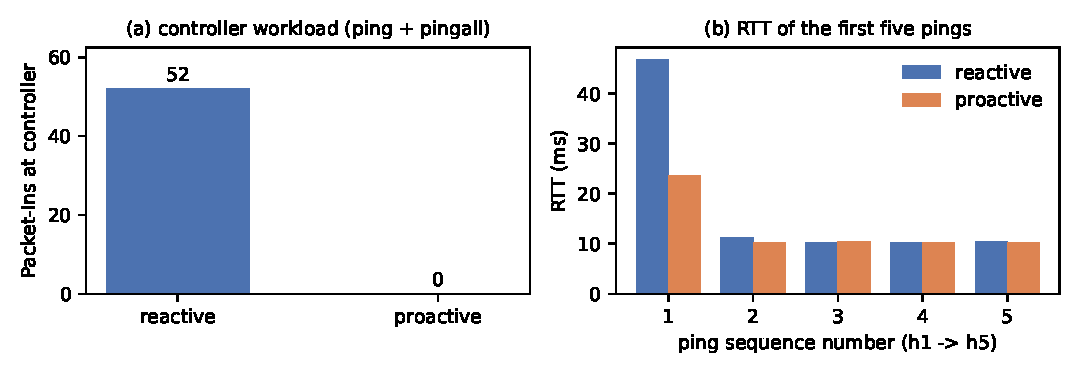
\includegraphics[width=\textwidth]{figs/p1.pdf}
\caption{Controller workload and the RTT of the first five pings h1 $\to$ h5.}
\end{figure}

\textbf{Reading the numbers.} The proactive s1 table already holds all eight rules before a single
packet is sent, and it never changes; the controller does not see one Packet-In. The reactive s1 table
starts with only the table-miss and IPv6 rules and grows to 14 learned rules during pingall. Every
one of those rules exists because a packet first went to the controller, which is where the 52
Packet-Ins in the Ryu log come from (28 on s1, 24 on s2).

\textbf{First packet vs.\ the rest.} Even the proactive first ping (23.7\,ms) is slower than the
later ones, because h1 has to resolve h5's MAC address with ARP first --- roughly one extra round
trip. The reactive first ping pays another $\sim$23\,ms on top of that: the ARP request, the ARP reply
and the first ICMP packets each go up to the controller (6 Packet-Ins for this exchange) before the
rules that would forward them exist. Once those rules are in place, forwarding is identical in both
cases, about 10.3\,ms, which is twice the 5\,ms link delay plus a little processing.

\textbf{The trade-off.} Reactive installation pays an initial forwarding delay for every new flow,
and its controller workload grows with the number of new flows. In exchange it only ever installs
rules for traffic that really exists, those rules expire on their own, and it copes with hosts it has
never seen. Proactive installation removes both the setup delay and the controller load, but only
because the topology and every host had to be known beforehand; it fills the table with rules
whether or not they are used, and if the network changes it does not adapt by itself.

% =====================================================================
\section{Part 2: Link-metric-based path selection}

\subsection{Topology and link metric}
The ring has one host per switch, h$i$ on port 1 of s$i$, and two possible paths between any two
opposite switches. The metric chosen is \textbf{delay}: the cost of a link is its one-way delay in
milliseconds, so a lower-delay link is cheaper.

\begin{table}[H]
\centering
\caption{Ring links (ports as numbered by Mininet in \texttt{addLink} order).}
\begin{tabular}{lcccc}
\toprule
Link & s1--s2 & s2--s3 & s3--s4 & s4--s1 \\
\midrule
Bandwidth & 2 Mbit/s & 2 Mbit/s & 1 Mbit/s & 1 Mbit/s \\
Delay: default / changed test & \textbf{20 / 40 ms} & 10 ms & 20 ms & 15 ms \\
Ports & s1:2 -- s2:2 & s2:3 -- s3:2 & s3:3 -- s4:2 & s4:3 -- s1:3 \\
\bottomrule
\end{tabular}
\end{table}

\subsection{Controller design}
\textbf{Switch-level topology.} \texttt{p2\_controller.py} uses Ryu's LLDP link discovery
(\texttt{-{}-observe-links}). Every discovered link is stored as a directed edge, mapping
\texttt{(src\_dpid, dst\_dpid)} to \texttt{(src\_port, dst\_port)}, which gives both the graph and
the port to use for each hop. The controller logs ``topology complete: 4 switches, 8 directed links'' once the
whole ring is known, and the experiment script waits for that line before sending traffic.

\textbf{Host attachment points.} A host is learned from the first ARP or IPv4 Packet-In that arrives
on a port that is \emph{not} an inter-switch port, giving \emph{IP $\to$ (MAC, switch, port)}.

\textbf{Path computation and rules.} The path is computed with Dijkstra over the directed edges, using
\texttt{link\_costs()} as the cost map. On the first IPv4 packet between two hosts the controller
installs \texttt{(ipv4\_src, ipv4\_dst) $\to$ out\_port} on every switch of the path (priority 10,
30\,s idle timeout), starting with the switch nearest the destination so the packet does not overtake
its own rules. The reverse direction is installed at the same time along the reversed path, which is
what makes connectivity work both ways. To make each decision explainable, the controller also logs
every loop-free candidate path with its cost breakdown.

\textbf{ARP in a ring.} Unlike Part 1, this topology has a loop, so flooding an ARP broadcast would
make it circulate forever. The controller therefore answers ARP requests itself whenever it already
knows the target (proxy ARP), and otherwise sends the request only out of host-facing ports, never into
the ring.

\textbf{Assumptions.} Hosts do not move (the first learned location is kept). Delays are the
configured link values --- OpenFlow has no way of reporting a link's delay --- and they are the same
in both directions, which is why the reverse path is simply the forward path reversed. Switch s$N$ has
datapath id $N$ (Mininet's default).

\subsection{Why this path is selected}
For h1 $\to$ h3 the two candidates are s1--s2--s3 and s1--s4--s3. The controller log for both tests:
\begin{Verbatim}
default (s1-s2 = 20 ms)                        changed (s1-s2 = 40 ms)
route 10.0.0.1 -> 10.0.0.3 (s1 -> s3)          route 10.0.0.1 -> 10.0.0.3 (s1 -> s3)
  candidate s1-s2-s3 : 20 + 10 = 30 ms <- chosen   candidate s1-s4-s3 : 15 + 20 = 35 ms <- chosen
  candidate s1-s4-s3 : 15 + 20 = 35 ms             candidate s1-s2-s3 : 40 + 10 = 50 ms
\end{Verbatim}
With the default values the route through s2 adds up to 30\,ms against 35\,ms through s4, so it wins
even though its first hop (20\,ms) is slower than s1--s4 (15\,ms) --- it is the total along the path
that counts. Raising s1--s2 to 40\,ms makes the s2 route cost 50\,ms, and the controller moves h1 $\to$
h3 to the s4 route, as expected.

\begin{figure}[H]
\centering
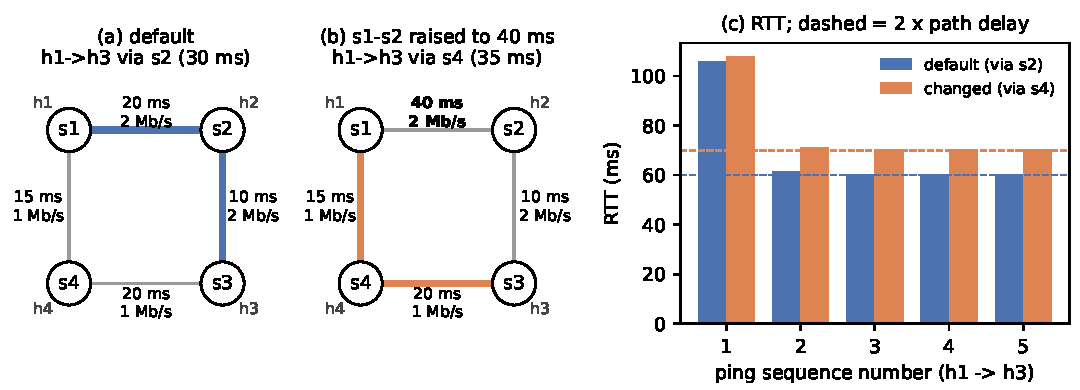
\includegraphics[width=\textwidth]{figs/p2.pdf}
\caption{Selected path for h1 $\to$ h3 in both tests, and the measured RTT of each ping.}
\end{figure}

\subsection{Evidence and performance}
Table~\ref{tab:p2flows} shows the rule for traffic 10.0.0.1 $\to$ 10.0.0.3 on each switch, taken from
\texttt{dump-flows} right after the first ping. In the default test s4 has no rule for this pair at
all; in the changed test s2 has none. The traffic therefore physically follows the path in the log.

\begin{table}[H]
\centering
\caption{Flow-table entry \texttt{ip,nw\_src=10.0.0.1,nw\_dst=10.0.0.3} on each switch.}
\label{tab:p2flows}
\begin{tabular}{lll}
\toprule
Switch & Default & Changed \\
\midrule
s1 & \texttt{actions=output:2} (to s2) & \texttt{actions=output:3} (to s4) \\
s2 & \texttt{actions=output:3} (to s3) & no rule \\
s4 & no rule & \texttt{actions=output:2} (to s3) \\
s3 & \texttt{actions=output:1} (to h3) & \texttt{actions=output:1} (to h3) \\
\bottomrule
\end{tabular}
\end{table}

\begin{table}[H]
\centering
\caption{Ping RTT h1 $\leftrightarrow$ h3 (performance measure).}
\begin{tabular}{llrrrrl}
\toprule
Test & Path & Path delay & Expected RTT & Measured RTT & h3 $\to$ h1 & pingall \\
\midrule
Default & s1--s2--s3 & 30 ms & 60 ms & \textbf{60.3 ms} & 60.3 ms & 0\,\% loss \\
Changed & s1--s4--s3 & 35 ms & 70 ms & \textbf{70.2 ms} & 70.4 ms & 0\,\% loss \\
\bottomrule
\end{tabular}
\end{table}

\textbf{Reading the numbers.} The measured RTT (pings 2--5) is twice the computed path delay almost to
the decimal, in both directions, so delay really is what the routing optimises. The first ping is
around 105\,ms in both tests because it also includes ARP resolution and the controller installing
the rules. In the changed test, staying on the old route would have given about 100\,ms; the
controller's choice gives 70\,ms.

% =====================================================================
\section{Part 3: Congestion-aware routing}

\subsection{Measuring utilization}
\texttt{p3\_controller.py} is a subclass of the Part 2 controller. Every second it sends an OpenFlow
port-statistics request to every switch. For a directed link u$\to$v it looks at \texttt{tx\_bytes} on
u's port towards v, takes the difference from the previous reply and divides it by the difference of
the switch-reported duration, which gives the rate actually sent onto the link. Utilization is that
rate divided by the link's bandwidth from the JSON file. Measuring per direction matters: a TCP flow
fills one direction with data while the other only carries ACKs.

\subsection{Congestion rule and flow handling}
A directed link whose utilization is above \textbf{70\,\%} counts as congested, and its cost becomes
\emph{delay + 100\,ms}; otherwise the cost is the Part 2 delay. Only \texttt{link\_costs()} is
overridden, so path computation, logging and rule installation are exactly those of Part 2. The
controller logs every link that becomes congested or clears.

The cost map is consulted only when a \textbf{new flow} is routed --- existing flows keep their path,
which the assignment allows. For that to be meaningful, Part 2's matching on \texttt{(ipv4\_src,
ipv4\_dst)} had to change: with it, a later flow between the same two hosts would simply hit the
existing rule and never reach the controller. Part 3 therefore matches each transport flow
(\texttt{ip\_proto}, both IPs and the TCP/UDP ports), so each new connection gets its own decision
based on the current measurements, and its rules disappear 30\,s after the flow ends.

For a fair baseline the same controller runs with \texttt{CONGESTION\_AWARE=0}: only the penalty is
switched off, so it routes exactly like Part 2, with the same per-flow rules and the same monitoring
in the log.

\subsection{Traffic scenario}
At $t=0$, \textbf{flow A} starts: UDP from h1 to h3 at 1.5\,Mbit/s for 30\,s. The network is idle, so
it is routed over the lowest-delay path s1--s2--s3 and loads s1$\to$s2 and s2$\to$s3 to about 81\,\%.
At $t=6$\,s, \textbf{flow B} starts: a new TCP connection from h1 to h3 for 15\,s. At $t=11$\,s the
TCP/UDP rules on all four switches are dumped. Throughput is measured at the receiver (iperf servers on
h3), not at the sender, because a sender counts data as sent as soon as it is queued.

\subsection{Results}
\begin{Verbatim}
aware   (p3_aware_ryu.log)                          static  (p3_static_ryu.log)
NEW FLOW TCP 10.0.0.1:51426 -> 10.0.0.3:5002        NEW FLOW TCP 10.0.0.1:51340 -> 10.0.0.3:5002
  congested links: s1->s2 82%, s2->s3 81%             congested links: s1->s2 81%, s2->s3 81%
                   (+100 ms each)                                      (ignored: static mode)
  candidate s1-s4-s3 : 15 + 20 = 35 ms   <- chosen    candidate s1-s2-s3 : 20 + 10 = 30 ms <- chosen
  candidate s1-s2-s3 : 120 + 110 = 230 ms             candidate s1-s4-s3 : 15 + 20 = 35 ms
\end{Verbatim}

\begin{table}[H]
\centering
\caption{TCP/UDP rules at $t = 11$\,s (A = UDP h1$\to$h3, B = TCP h1$\to$h3).}
\begin{tabular}{lll}
\toprule
Switch & Static & Congestion-aware \\
\midrule
s1 & A $\to$ output:2, B $\to$ output:2 (both to s2) & A $\to$ output:2 (s2), \textbf{B $\to$ output:3 (s4)} \\
s2 & A and B & A only \\
s4 & no TCP/UDP rule & B only \\
s3 & A and B $\to$ output:1 (h3) & A and B $\to$ output:1 (h3) \\
\bottomrule
\end{tabular}
\end{table}

\begin{table}[H]
\centering
\caption{Static vs.\ congestion-aware routing, measured at the receiver.}
\begin{tabular}{lrr}
\toprule
Measure & Static routing & Congestion-aware \\
\midrule
Path of the new flow B & s1--s2--s3 (shared with A) & s1--s4--s3 \\
\textbf{Throughput of flow B (TCP)} & \textbf{0.37 Mbit/s} & \textbf{0.87 Mbit/s} \\
Loss of flow A (UDP) & 9.8\,\% & 0\,\% \\
\bottomrule
\end{tabular}
\end{table}

\begin{figure}[H]
\centering
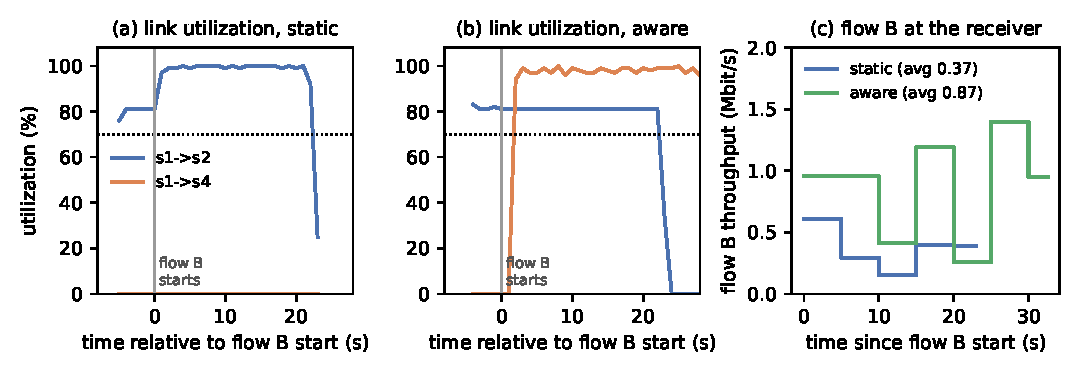
\includegraphics[width=\textwidth]{figs/p3.pdf}
\caption{Utilization of the two links leaving s1, from the controller's own measurements, and
throughput of flow B per 5\,s interval at the receiver. Dotted line: the 70\,\% threshold.}
\end{figure}

\textbf{The controller's decision.} Both controllers see the same thing when B arrives: s1$\to$s2 and
s2$\to$s3 at about 81\,\%. The static controller ignores it and gives B the 30\,ms path that A is
already filling. The congestion-aware controller adds 100\,ms to each of the two congested links, so
the s2 route now costs 230\,ms against 35\,ms through s4, and B is placed on the idle path. Flow A is
not touched. Figure 3 shows the consequence directly: with static routing s1$\to$s2 jumps to 100\,\%
the moment B joins it, while with congestion-aware routing s1$\to$s2 stays at A's 81\,\% and B fills
the previously unused s1$\to$s4 instead.

\textbf{Reading the numbers.} Under static routing B has to squeeze into the $\sim$0.4\,Mbit/s that A
leaves on a 2\,Mbit/s link, and reaches 0.37\,Mbit/s; A loses packets as well, because the two flows
now share one queue. On the other path B gets almost the whole 1\,Mbit/s link, 0.87\,Mbit/s, which is
2.4 times more, and A sees no loss. Across repeated runs B always got 0.85--0.88\,Mbit/s with the
congestion-aware controller and 0.17--0.42\,Mbit/s with the static one. Note that the alternative
path has only half the bandwidth --- the controller does better not because the s4 path is faster in
general, but because it is \emph{free}.

\subsection{Limitations}
The main limitation is that \textbf{existing flows are never moved}. A stays on its path for its whole
lifetime even if a better path appears, and only flows that start later benefit.

There is also \textbf{no damping}: the rule uses a single one-second sample and a hard threshold. A flow
whose rate hovers around 70\,\% could make consecutive new flows alternate between paths. Averaging
over several samples or using two thresholds (hysteresis) would avoid this.

Finally, \textbf{rerouted traffic creates new hotspots}. B itself pushes s1$\to$s4 to $\sim$97\,\%, so
a third flow would find both paths congested; the penalty then cancels out and the decision falls back
to plain delay.

\textbf{A note on measurement noise.} In some runs, in both modes, one 5\,s interval of flow A shows a
short loss burst. Port counters, topology and ARP were all quiet at that moment, so it comes from the
Mininet hosts briefly pausing inside WSL2, not from routing; hence we compare whole-run averages.

\end{document}
